\documentclass{article}
\usepackage{epsfig,url,amsmath}
\usepackage{graphicx,caption,subcaption,comment,color}

\begin{document}
\begin{center}
\Large
{\bf Getting Started Using Python}
\normalsize
\end{center}

The purpose of the following notes is to help you get started using python for your lab exercises and homework assignments. Although there are many python installations available, one of the easiest way to install python on your machine is by using Anaconda from Continuum Analytics. You can download the installation package from \url{https://www.continuum.io/downloads}. Make sure you use python version 2.7 installation (instead of version 3.5). 

\section{Python Interpreter}

A Python interpreter is used to execute your Python code. There are many ways to invoke the Python interpreter. First, you can write your python program and save it in a file with an extension \texttt{*.py}. For example, using your favorite text editor, you can write the following code and save it in as \url{hello.py} on one of the CSE machines, say, on \url{arctic.cse.msu.edu}

\begin{verbatim}
#!/usr/bin/python

print "Hello world!"
\end{verbatim}
Change the file permission so that it is executable (\texttt{chmod 700 filename}) and run the python program from the command prompt as follows:
\begin{verbatim}
    arctic>  cat hello.py
    #!/usr/bin/perl
    
    print "Hello world!"
    
    arctic> chmod 700 hello.py
    arctic> python hello.py
    Hello world!
\end{verbatim}

\section{IPython and IPython Notebook}

IPython provides an interactive shell that allows users to execute their python code in a user-friendly environment.
The following is a step-by-step approach you can use to launch ipython. The example given below is for Windows environment, though the steps are similar for Mac environment:
\begin{enumerate}
\item Launch Anaconda. You should be able to see the Anaconda prompt in the diagram as shown below:
\begin{figure}[h!]
\centering
  % Requires \usepackage{graphicx}
  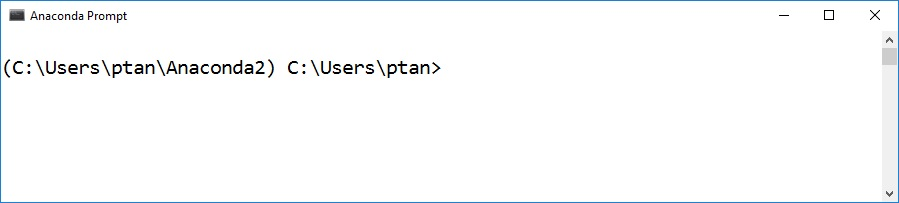
\includegraphics[width=3.8in]{anaconda.jpg}\\
\end{figure}
\newpage
\item Type ipython on the command prompt and it will launch an interactive shell as shown in the diagram below:
\begin{figure}[h!]
\centering
  % Requires \usepackage{graphicx}
  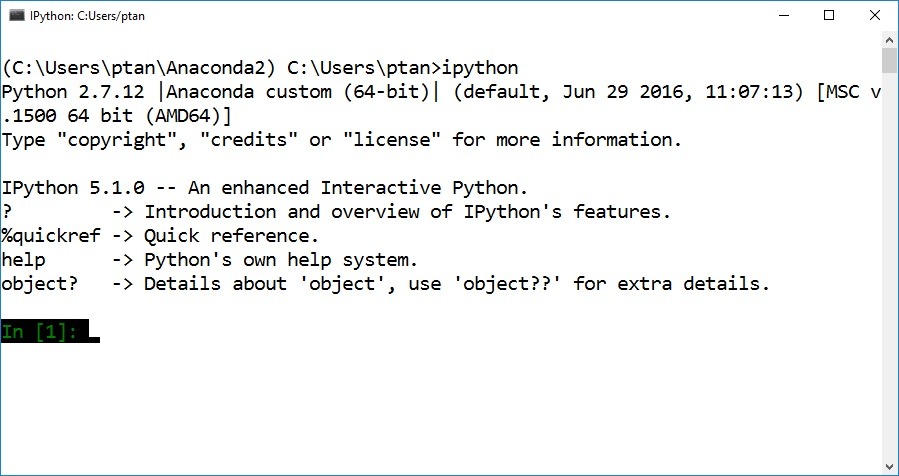
\includegraphics[width=3.8in]{ipython.jpg}\\
\end{figure}
\end{enumerate}

IPython notebook is an HTML-based user-friendly environment for running python code. To launch IPython notebook, type the following command:
\begin{verbatim}
(C:\Anaconda2) > ipython notebook
\end{verbatim}
This command will launch your Web browser and display the following page:
\begin{figure}[h!]
\centering
  % Requires \usepackage{graphicx}
  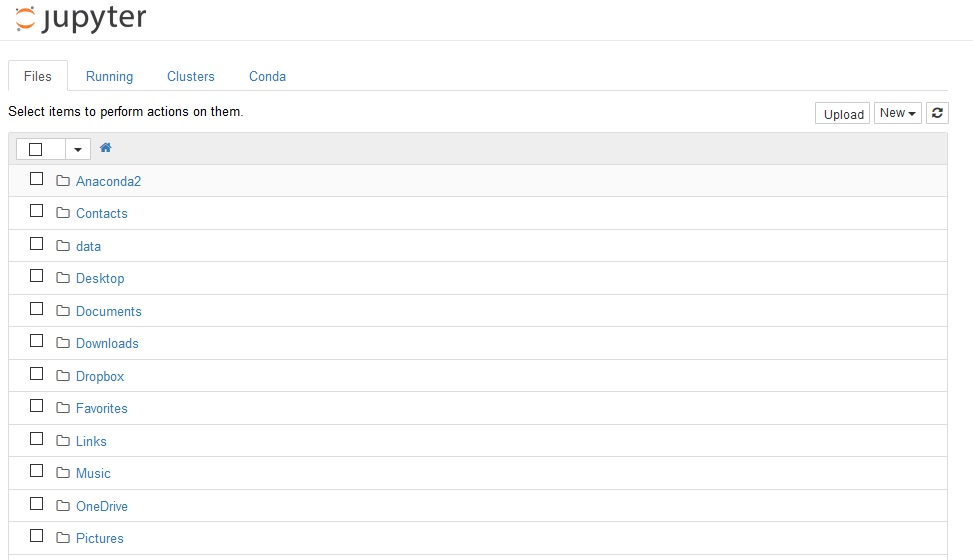
\includegraphics[width=4.5in]{notebook.jpg}\\
\end{figure}
\newpage

Click on the ``New" button on the top right hand corner of the web page and select ``Python" notebooks. The following web page will be rendered and the notebook is ready to accept new Python commands:
\begin{figure}[h!]
\centering
  % Requires \usepackage{graphicx}
  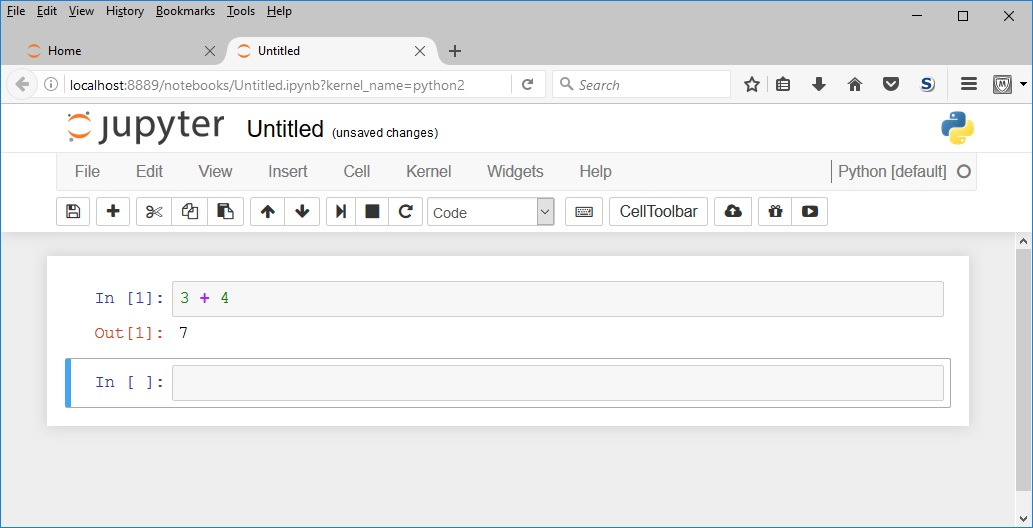
\includegraphics[width=4.5in]{notebook2.jpg}\\
\end{figure}

You can save the workspace by clicking on the ``File" and ``Save and Checkpoint" menu option as shown in the diagram below.

\begin{figure}[h!]
\centering
  % Requires \usepackage{graphicx}
  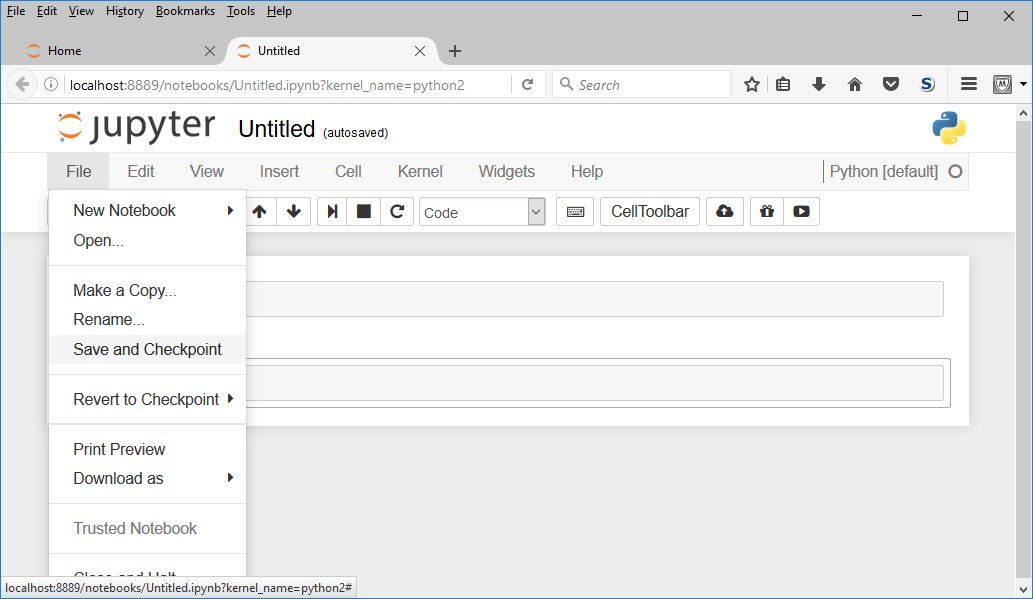
\includegraphics[width=4.5in]{notebook3.jpg}\\
\end{figure}




\end{document}